
\subsection{Finding a unifying data model and query language}

In any database system, the data model describe how data is represented within the database. Data in any database system must be organized logically according to the constraints imposed by the data model. When the data to be stored does not naturally fit within the data model, then it has to be changed to some form which respects the constraints. For example, a set of customer entities along with their individual lists of preferences is typically modeled as a list of \texttt{Customer} objects with a \texttt{List<Preference>} attribute in any typical object oriented programming language. However, such a list cannot easily fit using the relational data model. In order to be represented within an RDBMS, such a structure is typically converted into two tables (one for customers and one for preferences) with foreign keys in the preferences table referring to primary keys in the customer table. On the other hand, semi-structured data models are capable of modeling naturally lists of lists. In a semi-structured DBMS such as MongoDB ~\cite{MongoDB2015}, a single ~\texttt{Customers} collection, in which each \texttt{Customer} document has a \texttt{preferences} attribute which corresponds to that customer's list of preferences, would suffice.

Likewise, in any database system the query language indicates how data can be read from (and written to) the database. The input (the database instance) and output (the query results) of a given query are both instances of the database's data model, as such the data model and query language of a data store are tightly connected. Some data stores (for example RDBMS) have a query language which only describes \emph{what} data from the database should be returned by a given query; those languages are said to be \emph{declarative}. Other data stores have a query language which also describes \emph{how} data should be fetched from the data store and are said to be \emph{procedural}.

A polyglot persistence system must provide a single answer to a query that may span multiple subsystems, in which case data from those subsystems has to be joined despite data model and query language differences.  A solution to this problem problem is to define a common data model such that any data value $v$ expressed in any other data model can be transformed into a data value $m(v)$ expressed in the common model. Once a common data model is found, a common query language suitable for this data model is used as well. All surveyed PP systems have adopted this approach, but the chosen common data model and query language varies among them.

Some solutions, such as the MaxStream federated query engine ~\cite{Botan2010}, have decided to use the relational model as their common data model. MaxStream tries to integrate relational databases and streaming engines. Streaming tuples being regular, it is straightforward to map them to relational tuples. The difficulty of integrating of the relational and streaming data model is that streams do not represent a finite set of data, but an infinite stream in constant evolution. The way MaxDB integrates streams is by considering windows (state of data stream over a period of time) as relational tables and joining those windows with tables from the RDBMS. Choosing the relational data model also allows MaxStream to reuse a existing federated SQL query engine (in their case, SAP's MaxDB) and extend it to allow support of continuous queries with windowing statements.

However, MaxStream does not support any of the NoSQL data stores, a number of which use a semi-structured data model. As we have seen above, the semi-structured data model can express data structure which the relational data model cannot, thus the relational data model is not an "easy fit" to represent semi-structured data. Cure \& al ~\cite{Cure2011} suggest an approach to accomplish using classical data integration techniques. First, they suggest constructing a target relational schema representing the data from the various subsystems. Then they suggest creating \emph{GAV (Global-As-View)} mapping assertions from the different subsystems to the target schema. A SQL query can now be formulated over the target schema, and Cure's system is tasked with converting the query into a set of native subsystem queries according to the mappings.

Other solutions decide to use a unifying semi-structured data model and query language. For example, the FORWARD ~\cite{Forward} system uses the SQL++ language and data model (also developed at UCSD) for integration. The SQL++ data model is a superset of JSON (JSON itself ~\cite{JSON} is a very popular semi-structured data model) with enriched values. The SQL++ query language is a SQL-like query language in which multi-level navigation and nested collections in a query's output. It also allows specifying configurations which describe the behavior of algebraic or logical operators, essentially allow SQL++ to "morph" into any semi-structured (or relational) query language. Therefore every subsystem collection can be modeled as a SQL++ relation, thus removing the need for a manually constructed target schema (the schema being simply the union of the schemas of the subsystems modeled in SQL++) and specifying manually mapping assertions.

Until now, every query language described was declarative. However, a number of specialized data stores (in particularly those coming from the NoSQL world) do not provide such an interface. Instead, they provides procedural application programming interfaces (APIs) either through a RESTful web interface or a programming language specific driver. SOS ~\cite{Atzeni2012} and ODBAPI ~\cite{Sellami2014} are two PP systems which target relational and NoSQL stores. They both provide 1) a unifying semi-structured data model which is in one-to-one correspondence with JSON and 2) a simple API (java-based for SOS and web-based for ODBAPI) with three essential primitives : \texttt{get}, \texttt{put} and \texttt{delete}, all of which have their equivalent in the underlying data stores. These approaches offer a light layer on top of NoSQL and relational data stores which is convenient for simple queries, but they fall short of offering complex query capabilities and optimization. 



% NoSQL data models can be easily to a semi-structured data model such as JSON.

%In Forward, a SQL++ query is decomposed into 


% The regularity of streaming tuples makes it easy to map them

% SmartCIS ~\cite{}, another streaming query processing engine. 

% They have extended SAP's MaxDB 
% Some prefer centering around the relational data model and mapping heterogeneous data models to a relational form, although they may use bridging languages. For example

% We distinguish three categories in which researchers have decided to classify their data models


% SmartCIS isn't such a good model for our use case.

% Explain the differences between the relational and semi-structured data model.

% Show Max Stream : Relational

% Show Cure : Relational

% Show Forward : Semi-structured

\subsection{Integration Architecture}

\begin{figure}
 \centering
  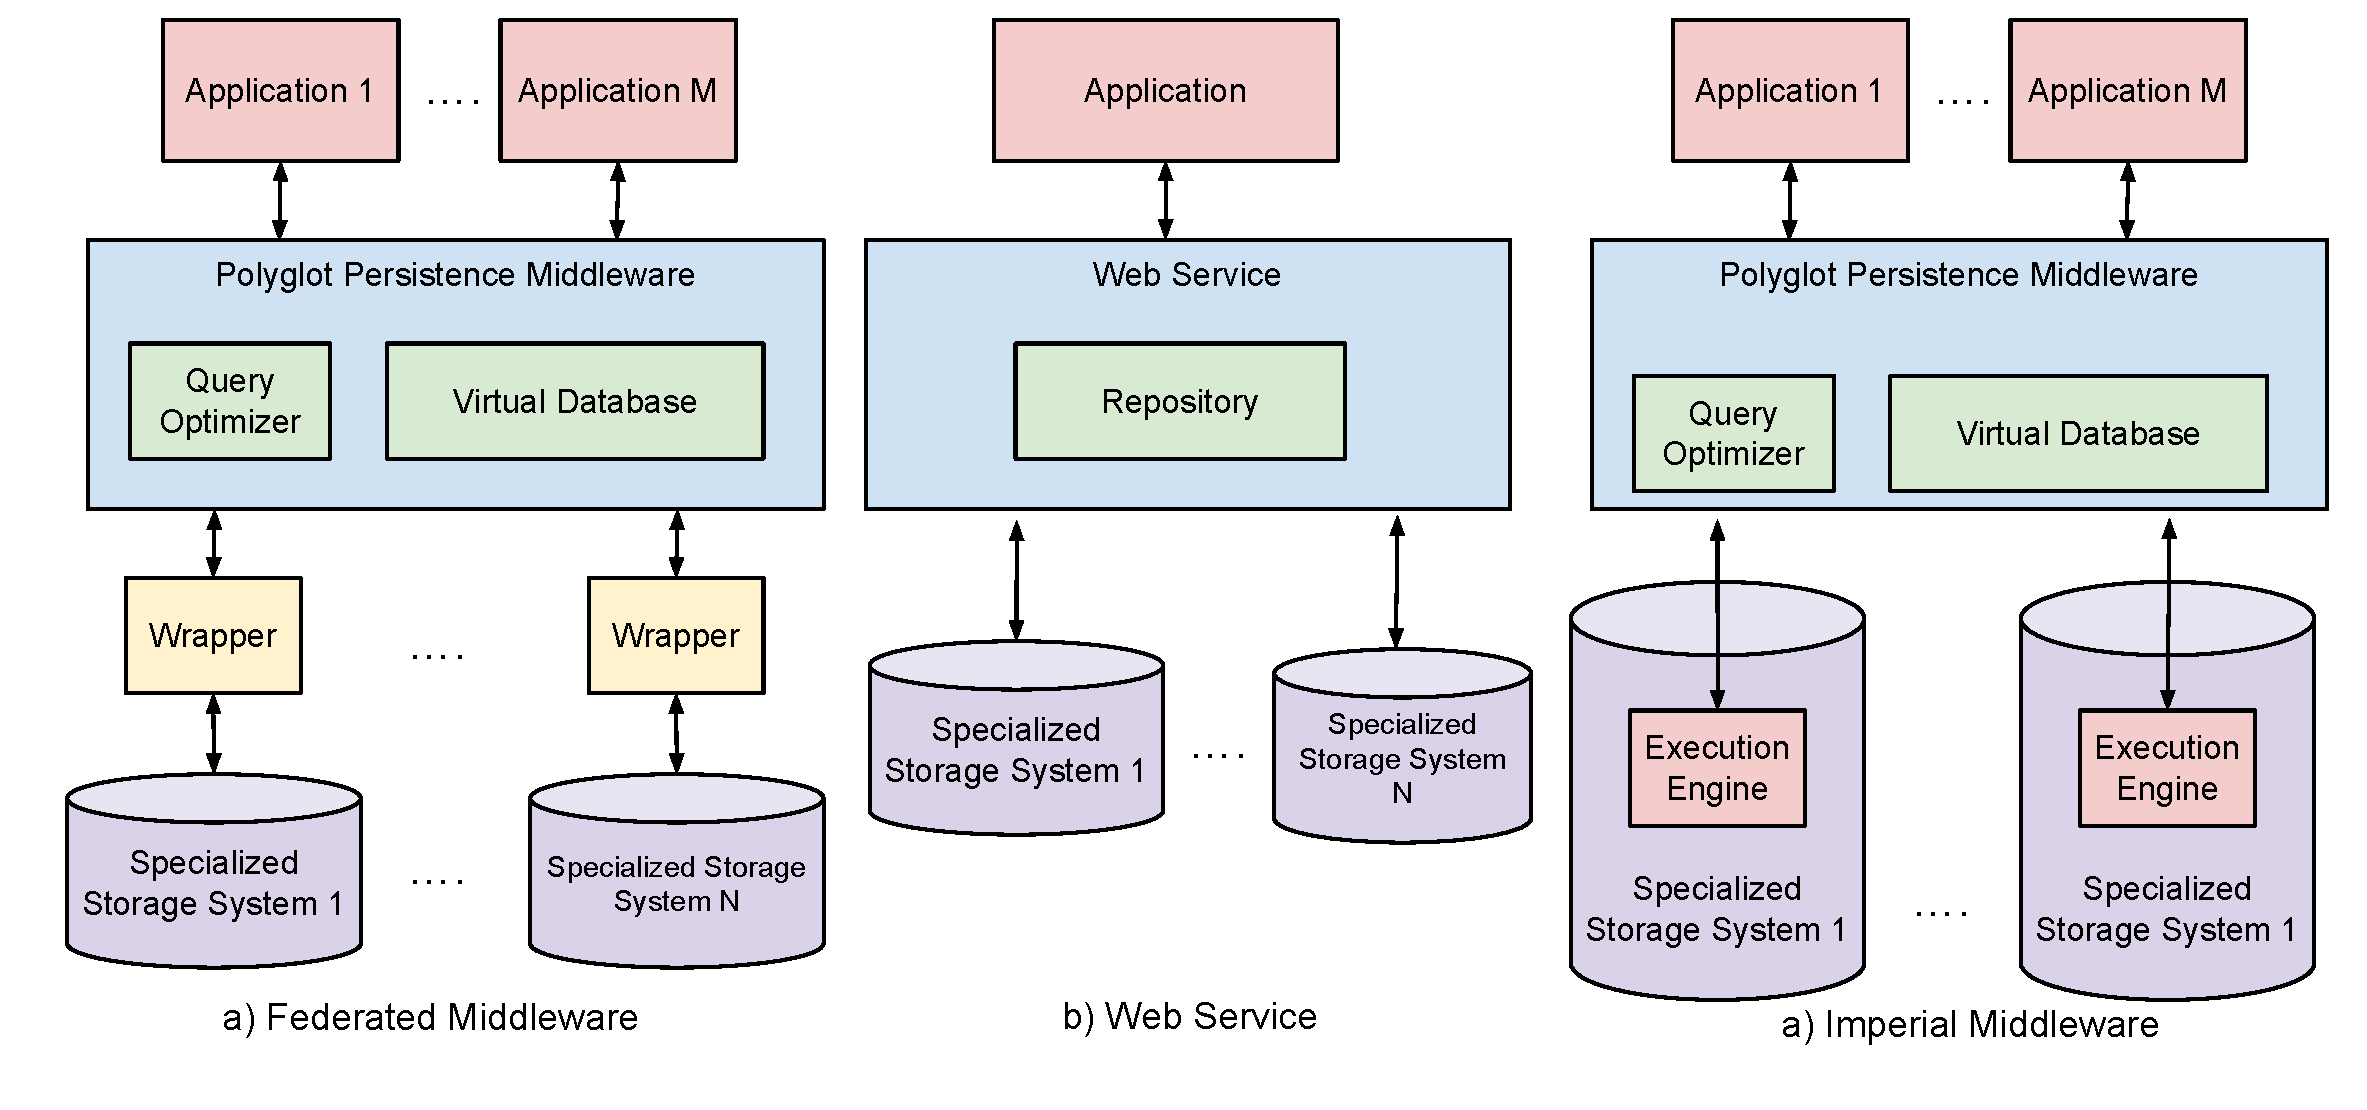
\includegraphics[width=1.1\textwidth]{images/MiddlewareArchitecture.pdf}
  \caption{An illustration of the different architectures for PP systems}
  \label{fig:architectures}
\end{figure}

A number of approaches exist to implement federated architectures. We identify three of them (shown on figure ~\ref{fig:architectures}) : the \emph{Federated Middleware}, \emph{Web Service} and \emph{Imperial Middleware} approaches.

\subsubsection{Federated Middleware Approach}

The problem of integrating data coming from multiple sources is a classical problem which has been extensively studied by the  data integration community ~\cite{Lenzerini2002}, and the federated middleware approach is the traditional way of accomplishing this as shown in the Garlic ~\cite{Carey95} and Tsimmis ~\cite{Chawathe94} data integration systems from the 1990's. In this architecture, the \emph{mediator} component (also called federated middleware) provides a query interface with which the client applications interact. From each input query an initial logical query plan gets created, which is then transformed (and possibly optimized) into a distributed query evaluation plan, in which subtrees of the plan (a.k.a subplans) are annotated with the subsystem on which they are expected to run. Each subplan is then sent to a source-specific wrapper component which translates it into a query native to the target subsystem, retrieves results and translates them back into the common data model. This is by far the most common approach used in the research community, being used by older data integration engines and newer polyglot persistence systems ~\cite{Ives2002} ~\cite{Borkar2006} ~\cite{Liu2010} ~\cite{Botan2010}  ~\cite{Atzeni2012} ~\cite{Sellami2014}. 

% The FORWARD query processor ~\cite{Forward} being developed at UCSD uses a federated architecture.

\subsubsection{Imperial Middleware Approach}

The imperial approach is similar to the federated approach but differs in how in interacts with the various subsystems. Instead of using querying the subsystems in their native query languages, it interacts with their execution engine directly, thus bypassing any query optimization that might have been used if the specialized systems was given instructions declaratively. This allows the mediator to fully control how a query will be executed and use query plans that even if not optimal locally (considering only one subsystem) are optimal globally. This approach has been followed by Lim ~\cite{Lim2013} in the Cyclops distributed stream processing system.

\subsubsection{Web Service Approach}

The idea of using web services for polyglot persistent solutions was first proposed by Martin Fowler ~\cite{Fowler2012}, and fully implemented as part of a Microsoft guide ~\cite{Sharp2013}. In the web service architecture, a dedicated web service is implemented to fulfill the storage needs of an application.  The application can then interact with the web service for all of its storage needs, typically through a RESTful interface, in which each query or update requires its dedicated RESTful endpoint. For each endpoint, the web service interacts directly with the various subsystems. It is possible for a single endpoint to interact with multiple subsystems, in which case data from multiple specialized systems is joined programmatically using object-oriented structures (i.e. Java classes) before being sent back to the client application.

The Web Service approach has significant drawbacks. It is a custom, "ad-hoc" solution : it is the application developer's responsibility to implement  the web service and to modify it whenever a new query or update needs to be formulated. It is also up to the developer to figure out what is the best distributed query plan formulation and how to manually join subsystem results since the web service has no optimizer or execution engine. Finally, a web service is can only serve applications it was designed for; a different application might need a new web service. Both the imperial and federated approach provides solutions yet they are not the widely accepted solution, especially in the software industry. We speculate that this is because the research tools which allow simultaneous access to SQL and NoSQL databases are only at their infancy and sufficient standards have not yet been established.

% One reason why to use a web service is that it can be configured for any set of specialized storage solution, including those for which state-of-the-art federated or imperial middlewares do not have wrappers for.

% Two types of components are typically used : a mediator (also called federated and wrappers.
% Users send queries to the mediator and those queries are then changed to 
% Federated Query Processor MiddleWare Architecture
% Most PP systems that have been studied focus on middle ware based architecture in which the user specifies a query which is then translated into sub components.
% Each sub component corresponding to a fragment which is sent to individual subsystems.
% These fragments are then translated into the subsystem's native query language and executed on those subsystems.
% The results of the fragment queries are then returned to the middleware which joins them together to form a response to the user initial query.
% This technique is inherited from the classical data integration integration problem that has been studied extensively in the 1990's.
% Describe first what is the global as view approach 

%\subsection{Defining the unifying interface}

%\subsubsection{Declarative Languages}

%Relevant papers : ~\cite{Lenzerini2002} ~\cite{Kirk1995} ~\cite{Katsis2009}
%~\cite{Srivastava2006} ~\cite{Tatbul2010} ~\cite{Botan2009} ~\cite{Botan2010} ~\cite{Lim2013}
%~\cite{Sharp2013} ~\cite{Cure2011} ~\cite{Atzeni2012} ~\cite{Sellami2014} ~\cite{Sellami2013}
%~\cite{Ong2014} ~\cite{Ong2015} ~\cite{Boag2010} ~\cite{Ives2002} ~\cite{Borkar2006}
%~\cite{Liu2010} ~\cite{Fowler2012}

%\subsubsection{Procedural Approaches}

% \reminder{Jules : In this section, we show what the generic, classical middleware query architecture looks like with the databases chosen above.}
 
 
 % MaxStream uses their own MaxStream Federator Language.
 
 \subsection{Synthesis}
 
 \begin{tabulary}{\linewidth}{ | L | C | C | L | }
\hline
	 & Declarative Vs Procedural & Data Models Supported & Integration Happens on \\ \hline
	AquaLogic XML Query Engine & declarative (XQuery) & XML, Relational, Web services & middleware (federated) \\ \hline
	FORWARD & declarative(SQL++) & NoSQL, NewSQL, SQL-on-Hadoop & middleware (federated) \\ 
\hline
	Microsoft Adventure Works & procedural & Key-Value, Graph, Document, Column Family, Relational & Web Service \\ \hline
	MaxStream & declarative(SQL with stream extension) & Relational, Various Stream data models & middleware (federated) \\ \hline
	SmartCIS & declarative (Stream SQL) & Relational, Stream & middleware (federated) \\ \hline
	Cyclops (DBMS+) & declarative ( SQL with stream extension) & Common Streaming Model & middleware (imperial) \\ \hline
	Cure \& al & declarative (SQL) & Document, Column-Family and Relational & middleware (federated) \\ \hline
	ODBAPI & procedural (REST API with unifying query language) & Document, Relational, Key-Value, Column-Family & middleware (federated) \\ \hline
	SOS Platform & procedural (REST API with unifying query language) & Document, Relational, Key-Value, Column-Family & middleware (federated) \\ \hline
\end{tabulary}




